\documentclass[a0paper, portrait]{baposter}
\usepackage{graphicx}
\usepackage[english]{babel}
\usepackage{calligra}
\usepackage[font=footnotesize, labelfont=bf]{caption}

\definecolor{headercol}{RGB}{0,129,216} %azul
%\definecolor{headercol2}{RGB}{216,87,0} % naranja oscuro 
%\definecolor{headercol2}{HTML}{FF9933}  % naranja feo
%\definecolor{headercol2}{HTML}{80C200} %verde
\definecolor{headercol2}{HTML}{B9E700} 

\begin{document}
\sffamily
\begin{poster}{
    % Poster Environment Options
    grid=false,
    columns=3,
    colspacing=0.75cm, % subject to change
    headerheight=0.1\textheight,
    background=plain,
    bgColorOne=white,
    eyecatcher=true,
    %Postbox environment options
    borderColor=black,
    headerColorOne=headercol2,
    headerColorTwo=headercol2,
    textborder = roundedsmall,
    headerborder=closed,
    headershape=roundedleft,
    headershade=plain,
%    headerFontColor = white,
    headerfont=\Large\sffamily\bfseries,
    boxshade=none,
    linewidth=0.10cm,    
}
  % Eye Catch
  { 
\includegraphics[height=0.1\textheight]{uanl.png} }
  % Title
  {
    \bf\sf Generation of Topic Tag Clouds
    %\bf\textsc{}}     
  }
     % Author
  {
    {\it Jes\'us Antonio Soto Vel\'azquez} \\
    \small {
    Undergraduate Program in Software Technology Engineering \\
    Faculty of Mechanical and Electrical Engineering, Universidad Aut\'onoma de Nuevo Le\'on \\
    May 2013        
    }
  }
  % Logo  
  {
    
\includegraphics[height=8.0em]{fime.pdf}
    \hspace{2.0em}
    
\includegraphics[height=8.0em]{ciidit.png}
  }

  %%
  %% Poster Content
  %%

  % BOX1
  \begin{posterbox}[name=intro, column=0, row=0]{Topic Visualization} {
    Tag clouds aid users to recognize at a first glance what a group of various documents is about by displaying the most relevant words or topics.
    
    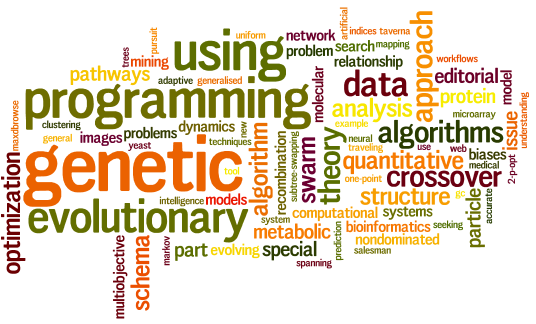
\includegraphics[width=\linewidth]{wordle2.png}
    \captionof{figure}{Artistic tag cloud using Wordle}
    \label{fig:1}
    
    \vspace{1em}The {\bf objective} is to deploy a web platform which generates tag clouds with meaningful information extracted from a collection of documents. This work focuses on such an insightful {\em visualization} of the topics in the documents. %while also considering possible interaction with the tag cloud to retrieve more information. % reword plz
  }
  \end{posterbox}

  %BOX2
  \begin{posterbox}[name=tech, column=0, below=intro]{Tackling the problem} {
    Several aspects were taken into account when choosing the right information to put in the tag cloud, such as: \newline
    \begin{description}
    \item[Stopword filtering] Unimportant words in the given context were discarded. Solved with {\em String matching algorithms \cite{Charras}}. 
    \item[Word stemming] Words with the same root were grouped together. Resolved with the {\em Snowball \cite{Porter} library}.
    \item[Language detection] Articles in other languages were to be excluded from the tag clouds. Resolved with the {\em language-detection \cite{Nakatani} library}.
    \item[The tag cloud] Manage structure and appearance of a tag cloud. Resolved with the {\em OpenCloud \cite{Mcavallo} Java library} 
    \item[Portability] As the intention was to reach as many users as possible, a web environment was chosen. Technologies used:{\em HTML5, CSS, Javascript, Servlets} 
    \end{description}
  }
  \end{posterbox}

  %BOX3
  \begin{posterbox}[name=initial, column=0, below=tech]{Initial solution} {
    The initial solution made use of OpenCloud, a Java library that aids the creation of tag clouds for the web. Using HTML and CSS, the tag cloud was given a simple styling and presentation. \\
    
    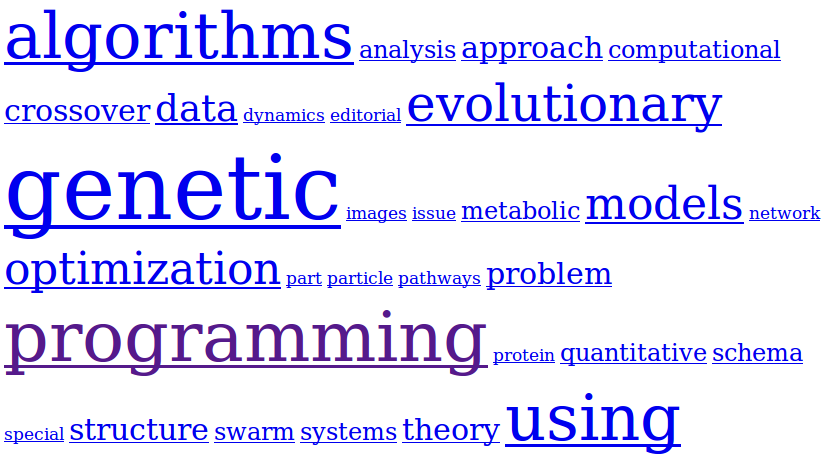
\includegraphics[width=\linewidth]{initial.png}
    \captionof{figure}{Tag cloud using OpenCloud}
    \label{fig:2}
  }
  \end{posterbox}

  %BOX4
  \begin{posterbox}[name=semantic, column=1, row=0]{Semantic approach} {
    Rather than focusing on the artistic side of tag clouds, like most tag cloud tools do, an approach on {\bf semantic similarity} between topics was taken. As such, the position of each topic is determined by the semantic similarity of itself and its surroundings.\\[3ex]
    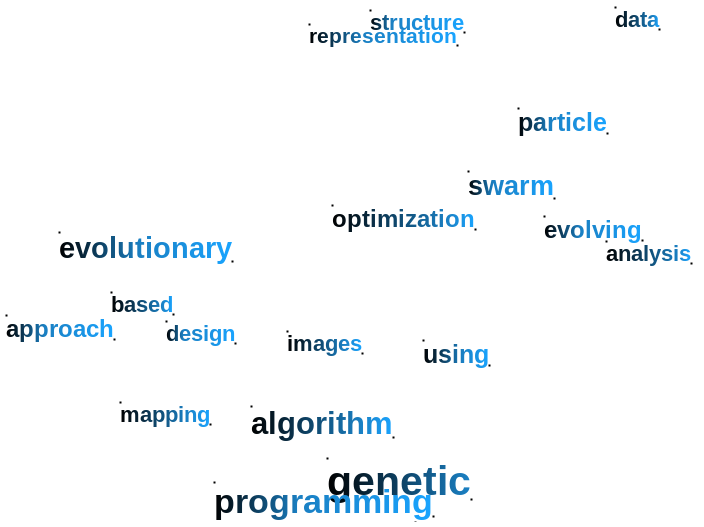
\includegraphics[width=\linewidth]{colors2.png}
    \captionof{figure}{Topic grouping with gradients\\}
    \label{fig:3}     
    \vspace{1.0em}It might be of interest knowing how active or inactive the topics have been throughout the years. For such cases, a {\bf two-color gradient} is used, such that the brighter the color, the more active it is. 
  }
  \end{posterbox}
  
  %BOX5
  \begin{posterbox}[column=1, name=index, below=semantic]{Indexing documents} {
    In order to quickly search through the documents by typing a keyword, a structure known as an index was used. The tool used to index the groups of articles, Solr, provides a simple interface between the data stored and the means of returning the desired information in a web environment. \\[3ex]
    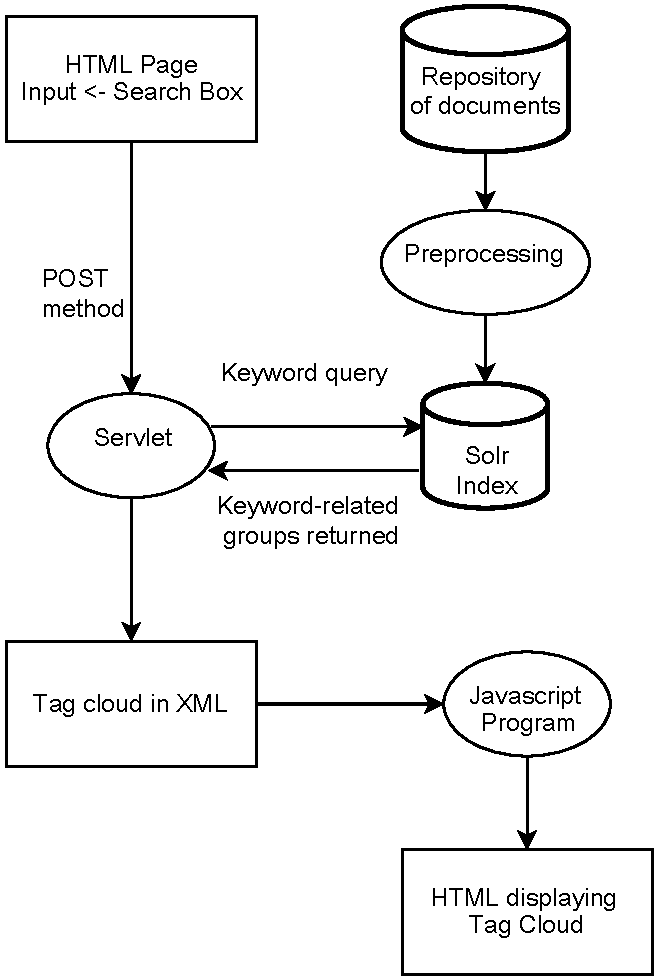
\includegraphics[width=\linewidth]{arch.pdf}
    \captionof{figure}{Overall Software Architecture}
    \label{fig:4}
    }
  \end{posterbox}

  %BOX6
  \begin{posterbox}[name=interact, column=2, row=0]{User interaction} {
    The first step to allow interaction with the tag cloud was through the functionality of clicking a word in the tag cloud and firing an event for that particular word. A match between the cursor's coordinates \cite{Lopez} and each of the words' coordinates is considered. %This was done by looking for a match of the cursor's coordinates and all of the words' coordinates. 
  }
  \end{posterbox}

  
  %BOX7
  \begin{posterbox}[column=2, name=future, below=interact] {Future Work} {
    The {\bf motivation} for creating {\em insightful} topic tag clouds has been shown, and a candidate {\bf architecture} to deploy a web platform with such functionality has been presented.  \\[3ex]
    Key points for further development are:
    \begin{description}
      \item[Data retrieval from tag cloud] Through user interaction, more information about the selected topic can be obtained, such as researchers involved.
      \item[Generation on the web] Given a document from the index in XML, a tag cloud should be generated.
      % \item I feel I'm missing something
    \end{description}
  }
  \end{posterbox}
  
  %BOX8
  \begin{posterbox}[column=2, name=ref, below=future] {References} {
      \small {
      \begin{flushleft}
        \bibliographystyle{ieee}
        \renewcommand{\section}[2]{\vskip 0.05em}
        \begin{thebibliography}{7}\itemsep=-0.1em 
          \setlength{\baselineskip}{0.4em}
          \bibitem{Apache}
            \newblock {\sc Apache Software Foundation}. {\it Apache Solr} 
            \newblock http://lucene.apache.org/solr/  
          \bibitem{Charras}
            \newblock {\sc Charras, Christian}; {\sc Lecroq, Thierry}. {\it Exact String Matching Algorithms}  
            \newblock http://www-igm.univ-mlv.fr/~lecroq/string/      
          %\bibitem{Garza}
            %\newblock {\sc Garza, Sara}. {\it Clustering of scientific articles.} 
            %\newblock http://elisa.dyndns-web.com/~saraelena/
          \bibitem{Lopez}            
            \newblock {\sc Lopez, Manuel.} {\it Get the coordinates of a mouse click on Canvas in Javascript}:
            \newblock http://miloq.blogspot.mx/2011/05/coordinates-mouse-click-canvas.html
          \bibitem{Nakatani}            
            \newblock {\sc Nakatani, Shuyo} @ Cybozu Labs, Inc. {\it language-detection Java Library} 
            \newblock https://code.google.com/p/language-detection/
          \bibitem{Mcavallo}
            \newblock {\sc Cavallo, Marco.} {\it Tag cloud Java library} 
            \newblock http://opencloud.mcavallo.org/ 
          \bibitem{Porter}        
            \newblock {\sc Porter, Martin}; {\sc Boulton, Richard}. Stemming Language {\em Snowball}. 
            \newblock http://snowball.tartarus.org/
        \end{thebibliography}
        \vspace{0.3em}       
      \end{flushleft}
      }
    }
  \end{posterbox}

  \begin{posterbox}[column=2, name=credits, below=ref] {Acknowledgements} {
      This poster was made under the supervision of Prof. Sara E. Garza and Prof. Elisa Schaeffer.\\
      They also provided the clusters of scientific articles grouped by their topics, as well as the functionality of setting the location of each of the tag words in a canvas. \\
      The author also wishes to thank SEP-PROMEP for its support (grant 103.5/12/7884).
    }
  \end{posterbox}

\end{poster}
\end{document}
